\documentclass[12pt]{article}
\usepackage[top=1in,left=1in, right = 1in, footskip=1in]{geometry}

\usepackage{graphicx}
%\usepackage{adjustbox}

\newcommand{\eref}[1]{(\ref{eq:#1})}
\newcommand{\fref}[1]{Fig.~\ref{fig:#1}}
\newcommand{\Fref}[1]{Fig.~\ref{fig:#1}}
\newcommand{\sref}[1]{Sec.~\ref{#1}}
\newcommand{\frange}[2]{Fig.~\ref{fig:#1}--\ref{fig:#2}}
\newcommand{\tref}[1]{Table~\ref{tab:#1}}
\newcommand{\tlab}[1]{\label{tab:#1}}
\newcommand{\seminar}{SE\mbox{$^m$}I\mbox{$^n$}R}

\usepackage{amsthm}
\usepackage{amsmath}
\usepackage{amssymb}
\usepackage{amsfonts}

\usepackage{lineno}
%\linenumbers

\usepackage[pdfencoding=auto, psdextra]{hyperref}

\bibliographystyle{chicago}
\usepackage{natbib}
\date{\today}

\usepackage{xspace}
\newcommand*{\ie}{i.e.\@\xspace}

\usepackage{color}

\newcommand{\Rx}[1]{\ensuremath{{\mathcal R}_{#1}}} 
\newcommand{\Ro}{\Rx{0}}
\newcommand{\RR}{\ensuremath{{\mathcal R}}}
\newcommand{\Rhat}{\ensuremath{{\hat\RR}}}
\newcommand{\tsub}[2]{#1_{{\textrm{\tiny #2}}}}
\newcommand{\dd}[1]{\ensuremath{\, \mathrm{d}#1}}

\newcommand{\comment}[3]{\textcolor{#1}{\textbf{[#2: }\textsl{#3}\textbf{]}}}
\newcommand{\jd}[1]{\comment{cyan}{JD}{#1}}
\newcommand{\swp}[1]{\comment{magenta}{SWP}{#1}}
\newcommand{\dc}[1]{\comment{blue}{DC}{#1}}
\newcommand{\hotcomment}[1]{\comment{red}{HOT}{#1}}

\newcommand{\jdnew}{\jd{NEW}}
\newcommand{\jddel}[1]{\jd{DELETE: #1}}

\begin{document}

\begin{flushleft}{
	\Large
	\textbf\newline{
	Predicting the impact of non-pharmaceutical interventions against COVID-19 on \textit{Mycoplasma pneumoniae} in the United States
	}
}
\newline
\\ 
Sang Woo Park\textsuperscript{1,2,*}, Brooklyn Noble\textsuperscript{3}, Emily Howerton\textsuperscript{1}, Bjarke F Nielsen\textsuperscript{4}, Sarah Lentz\textsuperscript{3}, Lilliam Ambroggio\textsuperscript{5}, Samuel Dominguez\textsuperscript{6}, Kevin Messacar\textsuperscript{6}, Bryan T Grenfell\textsuperscript{1}
\\
\bigskip
\textbf{1} Department of Ecology and Evolutionary Biology, Princeton University, Princeton, NJ, USA
\\
\textbf{2} Department of Ecology and Evolution, University of Chicago, Chicago, IL, USA
\\
\textbf{3} bioMérieux, Salt Lake City, Utah, USA
\\
\textbf{1} Department of Ecology and Evolutionary Biology, Princeton University, Princeton, NJ, USA
\\
\textbf{4} High Meadows Environmental Institute, Princeton University, Princeton, New Jersey, USA
\\
\textbf{5} Department of Pediatrics, Sections of Emergency Medicine and Hospital Medicine, University of Colorado School of Medicine and Children's Hospital Colorado, Aurora, CO, USA
\\
\textbf{6} Department of Pediatrics, Section of Infectious Diseases, University of Colorado School of Medicine and Children's Hospital Colorado, Aurora, CO, USA
\\
\bigskip

*Corresponding author: swp2@uchicago.edu
\bigskip
\end{flushleft} 

\section*{Abstract}
The introduction of non-pharmaceutical interventions (NPIs) against COVID-19 disrupted circulation of many respiratory pathogens and eventually caused large, delayed outbreaks, owing to the build up of the susceptible pool during the intervention period.
In contrast to other common respiratory pathogens that re-emerged soon after the NPIs were lifted, longer delays ($>$ 3 years) in the outbreaks of \textit{Mycoplasma pneumoniae} (Mp), a bacterium commonly responsible for respiratory infections and pneumonia, have been reported in Europe and Asia.
As Mp cases are continuing to increase in the US, predicting the size of an imminent outbreak is timely for public health agencies and decision makers.
Here, we use simple mathematical models to provide robust predictions about a large upcoming Mp outbreak in the US.
Our model further illustrates that NPIs and waning immunity are important factors in driving long delays in epidemic resurgence.

\pagebreak

\section{Introduction}

\textit{Mycoplasma pneumoniae} (Mp) is the most commonly detected bacterium for lower tract respiratory infections in children and adults \citep{waites2004mycoplasma,jain2015community,jain2015community2,bajantri2018mycoplasma}.
Mp pneumonia can affect a patient for a long period due to its long incubation period and long prodromal duration of symptoms, especially among children and high risk individuals.
For instance, outbreaks in schools have resulted in increased hospitalization, ventilator-associated pneumonia, severe extrapulmonary disease (e.g. Stevens-Johnson syndrome) and have been shown to last for several months \citep{walter2008community,olson2015outbreak}.
Increasing levels of macrolide-resistant Mp strains further highlight the importance of appropriate diagnosis and treatment \citep{pereyre2016mycoplasma}.

Multiannual cycles in Mp outbreak patterns have been observed in many countries, with large outbreaks occurring every 3--7 years \citep{kim2009mycoplasma,brown2016mycoplasma}.
Several potential mechanisms have been proposed to explain the observed epidemic cycles, including waning immunity \citep{omori2015determinant} and strain dynamics \citep{kenri2008genotyping,zhang2019positively}.
More parsimoniously, multiennial epidemic dynamics can also arise from simple, seasonally-forced immunizing epidemic dynamics, especially given low transmission rates \citep{earn2000simple,keeling2001seasonally}.

Along with other endemic viruses and bacteria, the circulation of Mp was disrupted in 2020 due to non-pharmaceutical interventions (NPIs) that were introduced to prevent the transmission of SARS-CoV-2 \citep{boyanton2024sars}.
The disruption of the expected epidemiological curve adds challenges to predicting future Mp outbreaks.
In contrast to other common respiratory pathogens that re-emerged within a year after NPIs were lifted, the re-emergence of Mp outbreaks has been delayed for more than 3 years in Europe and Asia \citep{sauteur2024mycoplasma}.
A long delay in epidemic resurgence is particularly alarming because it can allow for a build up of a large susceptible population, increasing the risk of a large outbreak as the infection resurges \citep{baker2020impact}.

As Mp infections are beginning to increase rapidly in the US (Figure 1A), predicting the size of an impending outbreak is critical for public health agencies and decision makers.
% The objective of this study was to predict Mp outbreaks using data from 2015 onward thereby providing critical data for clinical providers and public health agencies. 
Here, we present a modeling analysis of Mp outbreaks in the US using data from 2015 onward and predictions for potential upcoming outbreaks and subsequent epidemic dynamics.

\section{Methods}

\subsection{Data}

We analyzed over 2.57 million BIOFIRE® Respiratory (RP1.7, RP2, and RP2.1) Panel (bioMérieux, Salt Lake City, Utah) multiplex PCR test results, 8678 of which had a positive detection of Mp \citep{poritz2011filmarray,leber2018multicenter,creager2020clinical}. 
These deidentified patient test results were captured from 127 US inpatient and outpatient facilities from January 1, 2015 to June 29, 2024 using BIOFIRE® Syndromic Trends, a cloud-based pathogen surveillance network for BIOFIRE® instruments. Further details regarding the dataset and test result collection and interpretation methods have been previously published \citep{meyers2018automated}.
We also analyzed time-series data of influenza-like illnesses (ILIs), which were downloaded the FluView website (\url{https://gis.cdc.gov/grasp/fluview/fluportaldashboard.html}), and time-series data of Google Mobility for the US, which were taken from a previous publication \citep{park2024predicting}.

\subsection{Incidence proxy}

As discussed previously, test positivity can give a biased view of disease circulation patterns \citep{goldstein2011predicting,kissler2020projecting,park2024predicting}. 
Specifically, since test positivity in hospitals reflects prevalence of infection among individuals exhibiting respiratory symptoms, an increase (or decrease) in circulations of other respiratory diseases can cause test positivity of Mp infections to decrease (or increase).
To mitigate this bias, we calculated an incidence proxy for Mp infections by multiplying weekly percentages of MP positives with weekly percentages of weighted ILIs.
Limitations and assumptions to using this incidence proxy are discussed in \cite{goldstein2011predicting}.
Comparisons of three time series (Mp positivity, ILI positivity, and incidence proxy) are provided in Supplementary Figure S1. 

\subsection{Mathematical modeling of Mp outbreaks}

To estimate the epidemic dynamics of Mp infections in the US, we fitted a seasonally-forced, deterministic Susceptible–Infectious–Recovered-Susceptible (SIRS) model to Mp time series data \citep{dushoff2004dynamical,shaman2010absolute}.
The SIRS model considers three compartments, each representing the current infection status of an individual: Susceptible, Infected, and Recovered.
We assumed a homogeneously mixed population, where infected individuals (I) transmit infection to susceptible individuals (S) at rate $\beta(t)$ and recover at rate $\gamma=1/3\,\textrm{weeks}$ \citep{omori2015determinant}.
Recovered individuals were assumed to return to a susceptible state at rate $\nu$, which we estimated by fitting the model to data.
Birth and death rates $\mu=1/80\,\textrm{years}$ were assumed to be equal to fix the population size.
In order to capture epidemic dynamics before and after NPIs were introduced, we extended the SIRS model by decomposing the transmission rate $\beta(t)$ into two separate terms: (1) a periodic term with a period of 1 year $\tsub{\beta}{seas}(t)$ that captures seasonal transmission, reflecting epidemic peaks in summer and fall (Figure 1A) and (2) a non-periodic, time-varying term that captures changes in contact patterns after the introduction of COVID-19 NPIs in March, 2020 $\delta(t)$:
\begin{equation}
\beta(t) = \tsub{\beta}{seas}(t) \delta(t),
\end{equation}
where $\delta < 1$ corresponds to reduction in transmission due to NPI effects.
For the period term, we estimated a separate transmission rate for each of the 52 weeks in a year, while constraining the smoothness using random-walk priors.
For the non-period term, we allowed $\delta(t)$ to vary every 4 weeks from March 2020 and assumed $\delta(t)=1$ prior to March 2020; we also assumed $\delta(t)=1$ for longer-term predictions (for $t$ outside the data range).
The model was fitted to incidence proxy using log-normal likelihood:
\begin{equation}
\log (\textrm{incidence proxy}) \sim \mathrm{Normal}(\log (\rho C(t)), \tsub{\sigma}{obs}),
\end{equation}
where $C(t)$ represents the model-predicted weekly incidence, $\rho$ represents the scaling factor, and $\tsub{\sigma}{obs}$ represents the residual standard deviation.
Typically, either Poisson or negative binomial likelihoods are used to model discrete case counts;
since incidence proxy is a continuous variable, we relied on the log-normal likelihood instead.
Parameter estimation was performed in a Bayesian framework using the Hamiltonian Monte Carlo algorithm through the R package rstan \citep{carpenter2017stan,rstan};
mathematical and statistical details are presented in Supplementary Materials.
The resulting posterior distribution was used to predict future Mp outbreaks by projecting the model forward.
As a sensitivity analysis, we tried fitting the model to test positivity rather than incidence proxy;
we also performed the analysis using the SIR model, which assumes that infection provides life-long immunity.

\subsection{Evaluating the impact of NPIs and waning immunity on the delays in re-emergence of Mp outbreak}

To evaluate the potential impact of NPIs on long delays on Mp outbreaks, we performed sensitivity analyses on how reduction in transmission affect the timing of Mp outbreak resurgence.
Specifically, we separately varied the strength and duration of NPIs by modulating the estimated NPI effects $\delta(t)$.
First, the strength of NPIs were modified by taking fold changes in transmission $\delta-1$ and scaling it by a factor of $\theta$ such that the resulting transmission rate corresponds to
\begin{equation}
\beta(t) = \tsub{\beta}{seas}(t) [1+\theta (\delta(t)-1)].
\end{equation}
Second, the duration of NPIs were modified by assuming $\delta = 1$ after the end date $\tsub{t}{end}$:
\begin{equation}
\beta(t) = \begin{cases}
\tsub{\beta}{seas}(t) \delta(t) & t <  \tsub{t}{end}\\
\tsub{\beta}{seas}(t) & t \geq \tsub{t}{end}
\end{cases}.
\end{equation}
We varied $\tsub{t}{end}$ between 2020--2024.
We note that we evaluate the effects of strength and duration of NPIs independently and do not explore their joint effects.
Finally, we varied the duration of immunity $1/\nu$ between 3--15 years to assess how waning immunity contributes to the timing of Mp outbreak resurgence.
For illustration purposes, all parameters are set to median values from the posterior throughout the analysis, except for the duration of immunity, which we allowed to vary in the final analysis.

\section{Results}

\begin{figure}[!ht]
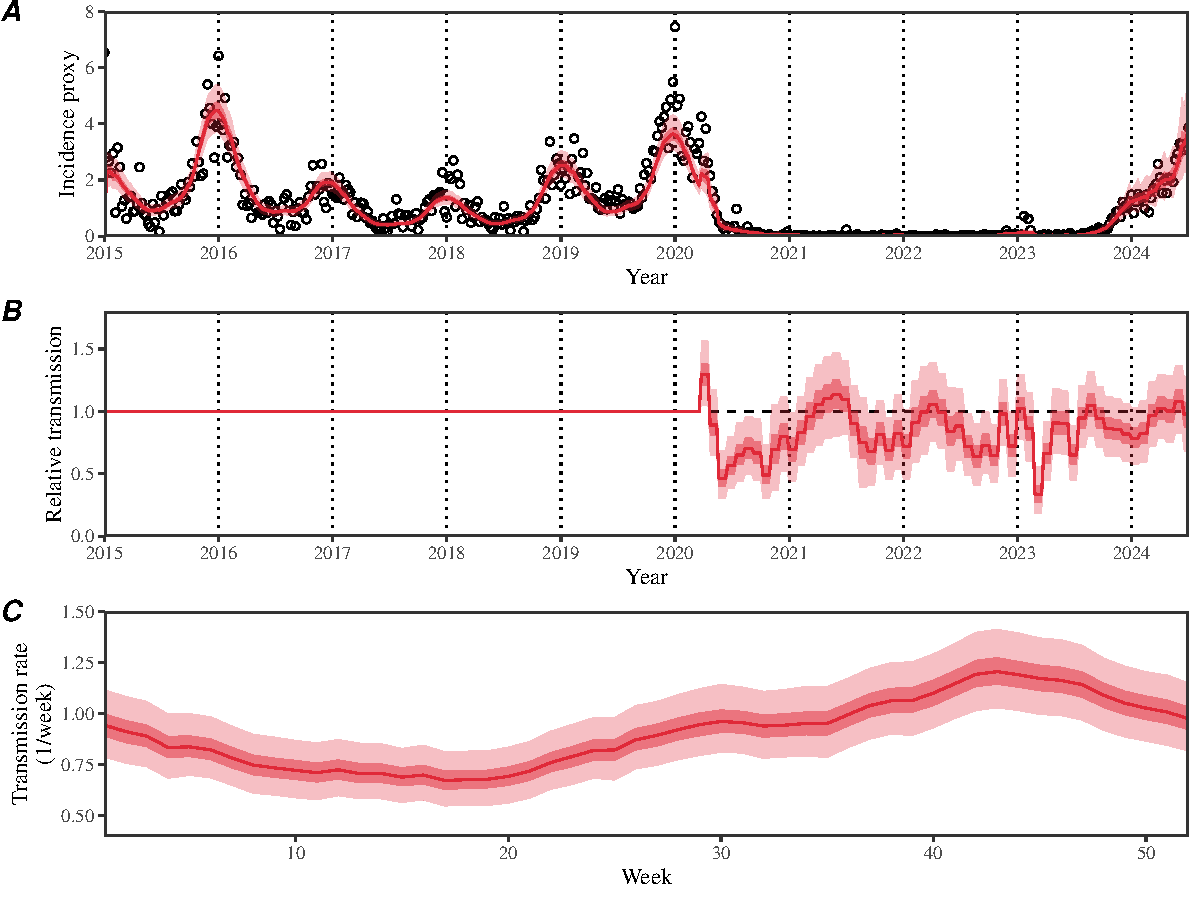
\includegraphics[width=\textwidth]{../figure1/figure1_new.pdf}
\caption{
\textbf{Summary of model fits to Mycoplasma pneumoniae incidence proxy in the US, 2015--2024.}
(A) Comparisons of observed (points) and fitted (line) trajectories of incidence proxy for Mp infections.
(B) Estimated non-periodic, time-varying transmission term, representing relative transmission $\delta$ following the introduction of NPIs; 
for example, 0.5 corresponds to a 50\% reduction in transmission.
(C) Estimated periodic transmission term  $\tsub{\beta}{seas}(t)$, representing seasonal transmission rate.
Red lines and shaded regions represent the estimated posterior median and corresponding 95\% and 50\% credible intervals.
}
\end{figure}

\textbf{Mathematical modeling of past Mp epidemics.}
The model reproduced the observed epidemic dynamics for Mp infections, including the seasonal and longer-term ($\approx 5$ year) epidemic cycles before NPIs were introduced and the delayed resurgence of the epidemic (Figure 1A).
To capture the response of Mp to the pandemic, the model required a strong reduction in transmission ($\delta(t) < 1$) in 2020 (Figure 1B).
The model further estimated sustained reduction in transmission for 2021--2023 (Figure 1C).
% We note that an increase in transmission predicted in Figure 1B must be interpreted with care as it also reflects the influx of imported infections from other countries (rather than increased transmission).
While we did not find a statistical correlation between the estimated changes in transmission and mean changes in Google mobility measures ($r=0.12$; 95\% CI: -0.04, 0.28),
the strength of correlation increased with lags, with strongest correlation occurring at a 4-week lag  ($r=0.36$; 95\% CI: 0.21--0.50; Supplementary Figure S2).
The model demonstrated typical sinusoidal patterns in seasonal transmission, peaking around week 43 (Figure 1C).
The model also estimated the mean duration of immunity to be 10.0 years (95\% CI: 8.6 years--11.2 years).
Comparisons between posterior and prior distributions are presented in Supplementary Figure S3.

% The SIR model gave nearly identical estimates for the NPI effects but underestimated the peak of the 2015 outbreak, providing support for the SIRS model (Supplementary Figure S2).

\textbf{Prediction of future Mp outbreaks.}
In line with other acute, partially immunizing respiratory pathogens \citep{baker2020impact}, the model predicted a large build-up of the susceptible pool during the NPI period (Figure 2A).
This build up of susceptible individuals could lead to a large Mp outbreak, which appears to have begun since the beginning of 2024 (Figure 1A);
the model forecasted that the epidemic would peak around the second half of 2024 and start to decline towards the end of 2024 (Figure 2B), reflecting decrease in transmission rate in winter (Figure 1C).
The peak incidence during this outbreak is estimated to be 4.3 (95\% CI: 3.5--5.2) times larger than previous peaks.
% The estimated peak incidence proxy is 2--3 times larger than the observed peak incidence proxy at the end of 2020.
The model further predicted that the outbreak beginning in 2024 would cause a large depletion of the susceptible pool (Figure 2A), which would lead to another delayed outbreak after several years (Figure 2B).

\begin{figure}[!th]
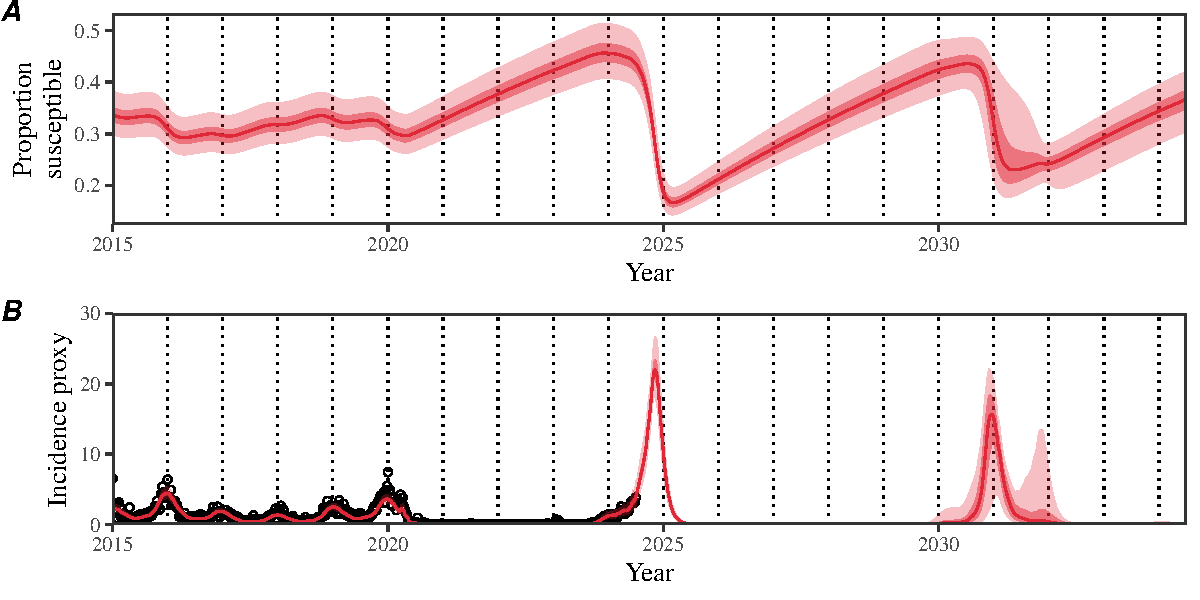
\includegraphics[width=\textwidth]{../figure2/figure2_new.pdf}
\caption{
\textbf{Predictions of future Mycoplasma pneumoniae outbreaks.}
(A) Predicted changes in the proportion of susceptible individuals.
(B) Predicted changes in weekly incidence proxy for Mp infections.
Red lines and shaded regions represent the estimated posterior median and corresponding 95\% and 50\% credible intervals.
Points represent the observed incidence proxy.
}
\end{figure}

\textbf{Impact of NPIs and waning immunity on the timing of Mp outbreak resurgence.}
The model predicted that a strong reduction in transmission due to NPIs is critical to explaining long delays in the Mp outbreak resurgence.
A smaller reduction in transmission (Figure 3A) would have led to more persistent epidemics as well as earlier resurgence of Mp outbreaks (Figure 3B).
Interestingly, the model still predicted a large outbreak in 2024 even when we assumed that NPI effects were 25\% weaker than what we originally estimated, demonstrating the risk of a susceptible build up.
Similarly, assuming shorter duration of NPIs (Figure 3C) led to earlier resurgence (Figure 3D).
However, even if transmission rates were to return to pre-pandemic values by the end of 2020, the model predicted that the resurgence would not be observed until 2022 (Figure 3D).
Finally, we found that the duration of immunity was also a key factor in determining the delays in Mp outbreak resurgences.
Faster waning of immunity would have caused a faster build up of the susceptible pool, leading to an earlier Mp outbreak.

\begin{figure}[!th]
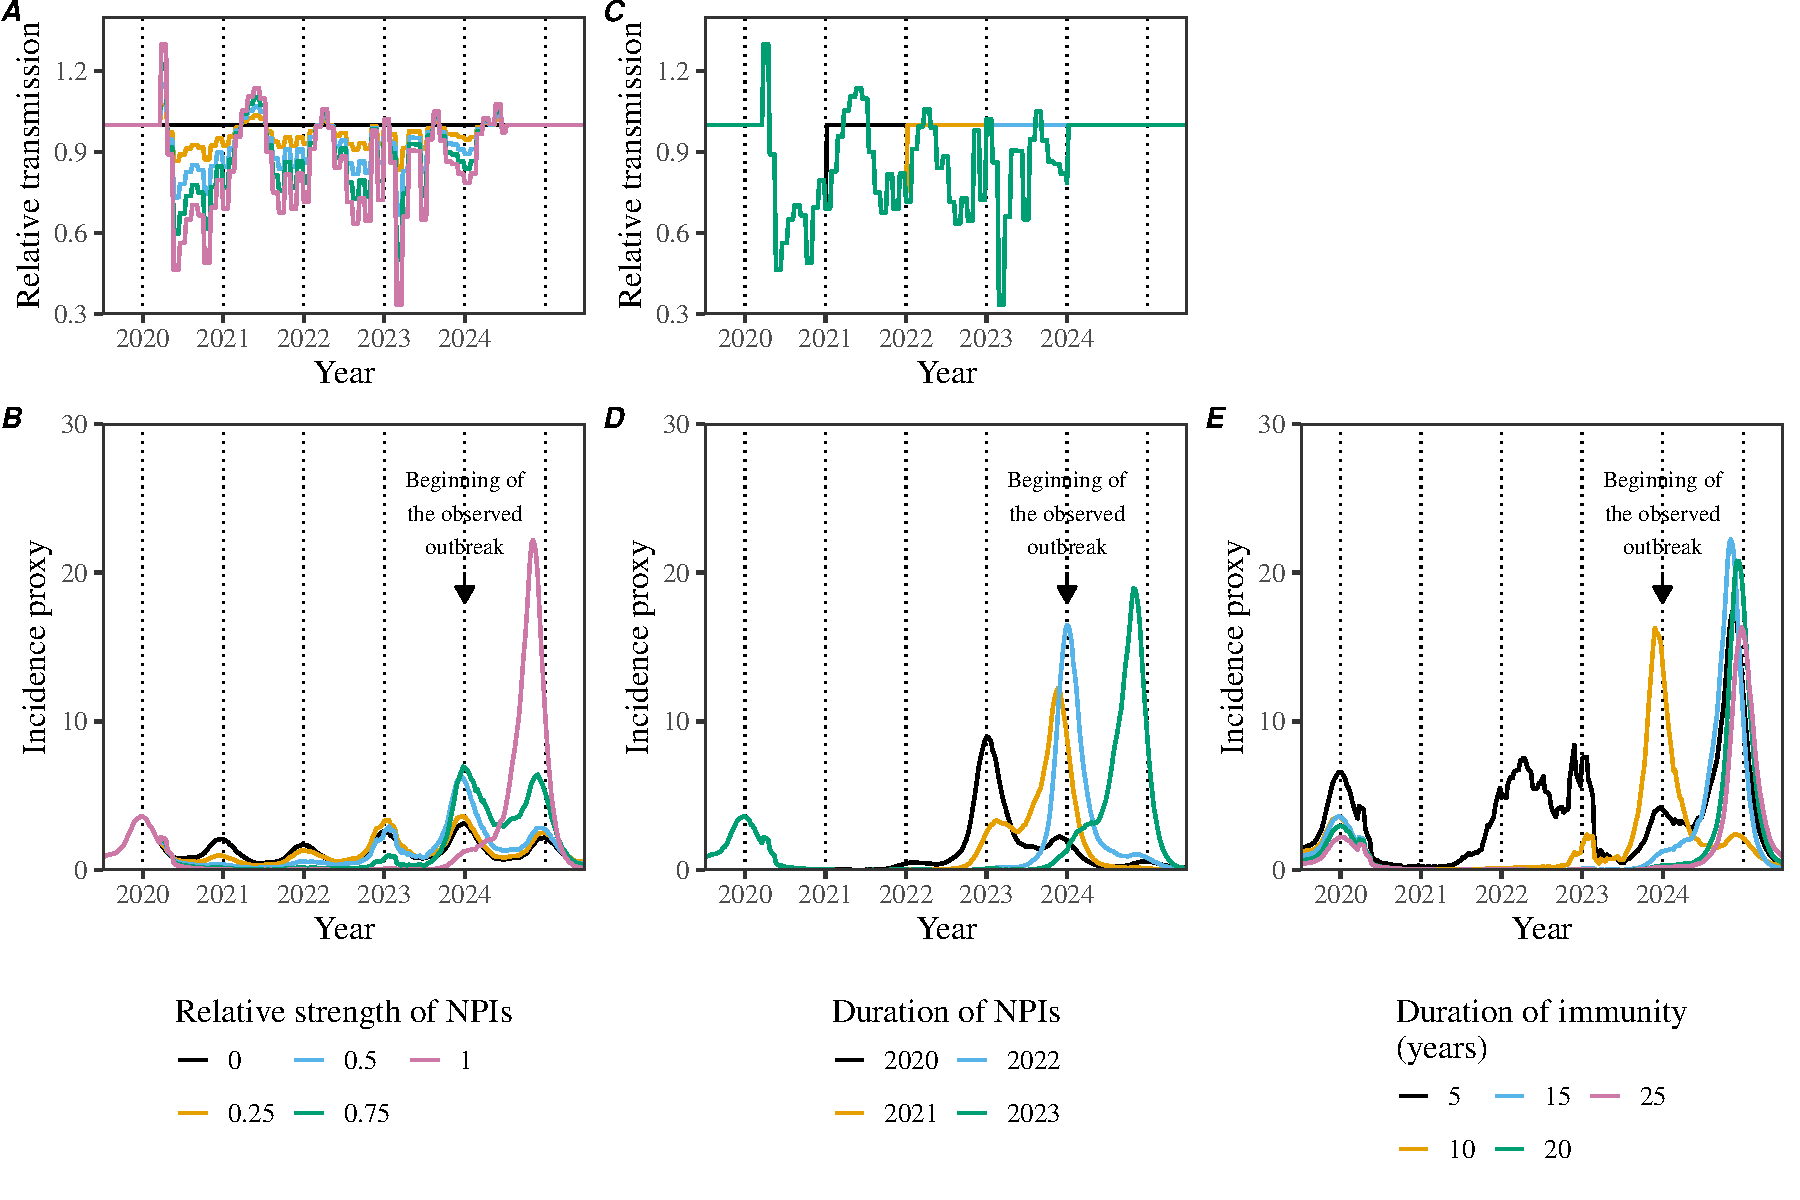
\includegraphics[width=\textwidth]{../figure3/figure3_new.pdf}
\caption{
\textbf{Impact of strength and duration of NPIs on the timing of Mp outbreak resurgence.}
(A, C) Assumed values for the relative transmission term $\delta$ following the introduction of NPIs by varying the strength (A) and duration (C) of NPIs.
(B, D) Resulting epidemic dynamics across different assumptions about NPIs.
(E) Resulting epidemic dynamics across different assumptions about the duration of immunity.
}
\end{figure}

\section{Discussion}

In this study, we investigated the impact of NPIs on future Mp outbreaks in the US.
By fitting a mathematical model to syndromic surveillance data, we predicted that a large Mp outbreak is imminent with a peak expected before the end of 2024.
The upcoming outbreak is expected to be much larger than past outbreaks and may last until the end of 2025; note, however, that there is currently substantial uncertainty associated with longer-term dynamics, including the duration of 2024--2025 outbreak and the timing of the subsequent outbreaks.
We can already observe what seems to be the beginning of this outbreak with an increasing rate of Mp detections throughout May and June 2024. 
Nonetheless, this prediction should alert clinicians and health care systems to be prepared for an increase in cases of pneumonia and potentially more rare presentations of Mp, such as reactive infectious mucocutaneous eruption (RIME) and encephalitis.

Our analysis highlighted the importance of strong reduction in transmission in explaining the delayed resurgence of Mp outbreaks.
Specifically, we estimated $\approx 50\%$ reduction in transmission in 2020, which is considerably larger than reduction in transmission estimated for other respiratory pathogens.
For example, \cite{baker2020impact} estimated a 20\% reduction in RSV transmission in the beginning of 2020.
Future studies should explore whether the epidemiology and life history of Mp infections cause its transmission to be more susceptible to behavioral changes.

% Our model relied on a simplifying assumption that infection provides life long immunity.
% In reality, serological and observational studies have indicated limited protection against reinfections, especially among children \citep{foy1983naturally}.
% Despite this simplifying assumption, the SIR model can give robust predictions as long as reinfections permit limited transmission, as illustrated by numerous studies across different childhood infections \citep{pons2018serotype,park2021epidemiological}.
% Moreover, parameter estimates from the SIRS model suggested a long duration of immunity, providing partial support for our current model.

% Previous study that showed that waning of immunity was necessary to explain multiannual cycles of Mp epidemics.
% In contast, we found that adding demographic stochasticity to the model was sufficient to reproduce complex epidemic cycles, suggesting that the waning of immunity may not be necessary to explain the observed pattern (\swp{SUPP}).
% More detailed data, especially on longitudinal serological information, would be needed to better understand the role of immunological factors in driving the epidemic dynamics of Mp infections.

There are several limitations to our study.
The dataset inherently contains a subset of the US population that has presented to a facility that utilizes the BIOFIRE® Respiratory Panel and participates in the BIOFIRE® Syndromic Trends network. As with many surveillance network data, this assumes inherent selection bias for less healthy individuals than the general population, therefore introducing the limitation of representativeness of the dataset. Additionally, due to the nature of deidentified data collection within the dataset, we are not able to conduct analyses based on patient or facility characteristics or account for variability in diagnostic testing algorithms between facilities. However, this dataset has evidenced correlation with other surveillance sources, reducing concern regarding representativeness and generalizability (Meyers et al., 2018). 

We did not account for heterogeneity in Mp dynamics across states as the quantity of data did not allow for reliable model-fitting at a regional scale.
We did not include age structure in the model as it would require more data.
% Breaking down the current data into four census regions suggest similarities in the epidemic patterns (\swp{SUPP}),
% We also did not account for changes in antibiotic uses, which can alter the susceptibility \citep{pereyre2016mycoplasma}
We also did not account for Mp strain dynamics, which have been hypothesized as another major driver of epidemic cycles \citep{kenri2008genotyping,zhang2019positively}.
Finally, our estimate of NPI effects need to be interpreted with care, especially during a period with very little case data;
the advantage of relying on a Bayesian framework is that these uncertainties can be captured and constrained using sensible priors.
Despite these limitations, our prediction that a build up of a susceptible pool over the past 4 years will cause a large Mp outbreak is likely qualitatively robust.

So far, there have been limited modeling studies analyzing epidemic dynamics of Mp infections \citep{omori2015determinant,zhang2019positively}. 
Our study reinforces recent work on the importance of understanding susceptible dynamics to predict the impact of perturbations to transmission \citep{baker2020impact,park2024predicting}.
% Preparing for the imminent Mp outbreak will be vital for hospitals and public health agencies in the US. 
As such, our analysis underlines the importance of serological surveillance data to capture the build up of the susceptible pool to foresee future outbreaks \citep{mina2020global,nguyen2022enterovirus}.
Our study also underlines the potential of BIOFIRE® Syndromic Trends network as a powerful surveillance measure.

\section*{Data availability}

All code is stored in a publicly available GitHub repository (\url{https://github.com/parksw3/mycoplasma_pred}).

\section*{Funding}

S.W.P. is a Peter and Carmen Lucia Buck Foundation Awardee of the Life Sciences Research Foundation.
B.F.N. receives funding from Carlsberg Foundation (grant no. CF23-0173).
K.M. receives funding as Principal Investigator of the NIAID Vaccine Research Center PREMISE EV-D68 Pilot Study.

\section*{Conflict of interest}

B.N. and S.L. are employees of bioMérieux. bioMérieux markets the BIOFIRE System and Syndromic Trends. 
BIOFIRE and FilmArray are registered trademarks of BIOFIRE Diagnostics LLC in the United States and/or other countries.
L.A's institution has received grant funding from Pfizer Inc. for an unrelated study.
S.D. receives grant support from BIOFIRE Diagnostics, DelveBio, and Karius; he is also a consultant for BIOFIRE Diagnostics, DelveBio, and Karius.

\pagebreak

\section*{Supplementary Text}
\setcounter{figure}{0}
\setcounter{equation}{0}
\renewcommand{\thefigure}{S\arabic{figure}}
\renewcommand{\theequation}{S\arabic{equation}}

\subsection*{Mathematical details}

Here, we used the standard SIRS model to capture the dynamics of Mp epidemics.
The dynamics of the model is governed by the following set of ordinary differential equations:
\begin{align}
\frac{\dd S}{\dd t} &= \mu + \nu R - (\beta(t) I + \mu) S\\
\frac{\dd I}{\dd t} &= \beta(t) SI - (\gamma + \mu) I\\
\frac{\dd R}{\dd t} &= \gamma I - (\nu+\mu) R
\end{align}
where $S$, $I$, and $R$ represents the proportion of individuals in a susceptible, infected, and recovered compartment;
$\beta(t)$ represents time-varying transmission rate;
$\gamma$ represents the recovery rate;
$\nu$ represents the immunity waning rate;
and $\mu$ represents the birth and death rates, which are assumed to equal to keep the population size fixed.
For simplicity, we assumed a population size of $S+I+R=1$.

We discretized the model using the Euler scheme outlined in \cite{he2010plug} at a weekly time scale $\Delta t = 1\,\mathrm{week}$:
\begin{align}
\Delta S(t) &= \left[1- \exp(-(\beta(t) I(t) + \mu) \Delta t )\right] S(t-\Delta t)\\
N_{SI}(t) &= \frac{\beta(t) I(t)\Delta S(t)}{\beta(t) I(t) + \mu} \\
\Delta I(t) &= \left[1- \exp(-(\gamma + \mu) \Delta t )\right] I(t-\Delta t)\\
N_{IR}(t) &= \frac{\gamma I(t)}{\gamma + \mu} \\
\Delta R(t) &= \left[1- \exp(-(\nu + \mu) \Delta t )\right] R(t-\Delta t)\\
N_{RS}(t) &= \frac{\nu R(t)}{\nu + \mu} \\
S(t) &= S(t-\Delta t) + \mu S - \Delta S(t) + N_{RS}(t)  \\
I(t) &= I(t-\Delta t) - \Delta I(t) + N_{SI}(t)  \\
R(t) &= R(t-\Delta t) - \Delta R(t) + N_{IR}(t)  \\
\end{align}
where $\Delta X(t)$ represents the total number of individuals leaving the compartment $X$ at time $t$,
and $N_{XY}(t)$ represents the number of individuals leaving the compartment $X$ to enter the compartment $Y$ at time $t$.
We calculated the incidence $C(t)$ by keeping track of the number of new infections in each week:
\begin{equation}
C(t) = N_{SI}(t).
\end{equation}
As explained in the main text, the transmission function was further decomposed into a periodic term $\tsub{\beta}{seas}(t)$ and a non-periodic, time-varying term $\delta(t)$:
\begin{equation}
\beta(t) = \tsub{\beta}{seas}(t) [1+\theta (\delta(t)-1)].
\end{equation}
Here, the periodic term $\tsub{\beta}{seas}(t)$ was modeled by estimating a weekly transmission rate for each of 52 weeks, which was modeled using cyclical, random-walk priors to allow for smoothing:
\begin{align}
\tsub{\beta}{seas}(t) &\sim \mathrm{Normal}(\tsub{\beta}{seas}(t-1), \sigma) \qquad t = 2 \dots 52\\
\tsub{\beta}{seas}(1) &\sim \mathrm{Normal}(\tsub{\beta}{seas}(52), \sigma)
\end{align}
A half-normal prior was used for the standard deviation in smoothing $\sigma$:
\begin{equation}
\sigma \sim \textrm{Half-Normal}(0, 0.2).
\end{equation}
The non-periodic term was modeled by estimating a separate $\delta$ for every four weeks with a normal prior centered around 1:
\begin{equation}
\delta(t) \sim \mathrm{Normal}(1, 0.2).
\end{equation}
Finally, we assumed a lognormal error model to fit the model to incidence proxy:
\begin{equation}
\log (\textrm{incidence proxy}) \sim \mathrm{Normal}(\log (\rho C(t)), \tsub{\sigma}{obs}),
\end{equation}
Here, $\rho$ represents the scaling factor and $\tsub{\sigma}{obs}$ represents the residual standard deviation.
For both terms, we used weakly informative half-normal priors to constrain the parameter space:
\begin{align}
\rho &\sim \textrm{Half-Normal}(0, 2)\\
\tsub{\sigma}{obs} &\sim \textrm{Half-Normal}(0, 0.5)
\end{align}
We also used a weakly informative prior for the duration of immunity $\tau = 1/\nu$ to prevent extremely long or short duration of immunity:
\begin{equation}
\tau \sim \mathrm{Normal}(300, 100).
\end{equation}
Finally, we assumed a uniform prior for the initial proportion susceptible $S(0)$ and a half-normal prior for the initial proportion infected $I(0)$:
\begin{align}
S(0) &\sim \mathrm{Unif}(0, 1)\\
I(0) &\sim \mathrm{Half-Normal}(0, 0.001)
\end{align}
The model was fitted using rstan \citep{carpenter2017stan,rstan} with 4 chains, each containing 8000 iterations.
Convergence was assessed based on the lack of warning signs from rstan, indicating: no divergent chains; no iterations exceeding maximum tree depth; sufficiently high Bayesian Fraction of Missing Information; sufficiently high effective samples sizes; and sufficiently low Rhat.

\pagebreak

\section*{Supplementary Figures}


\begin{figure}[!ht]
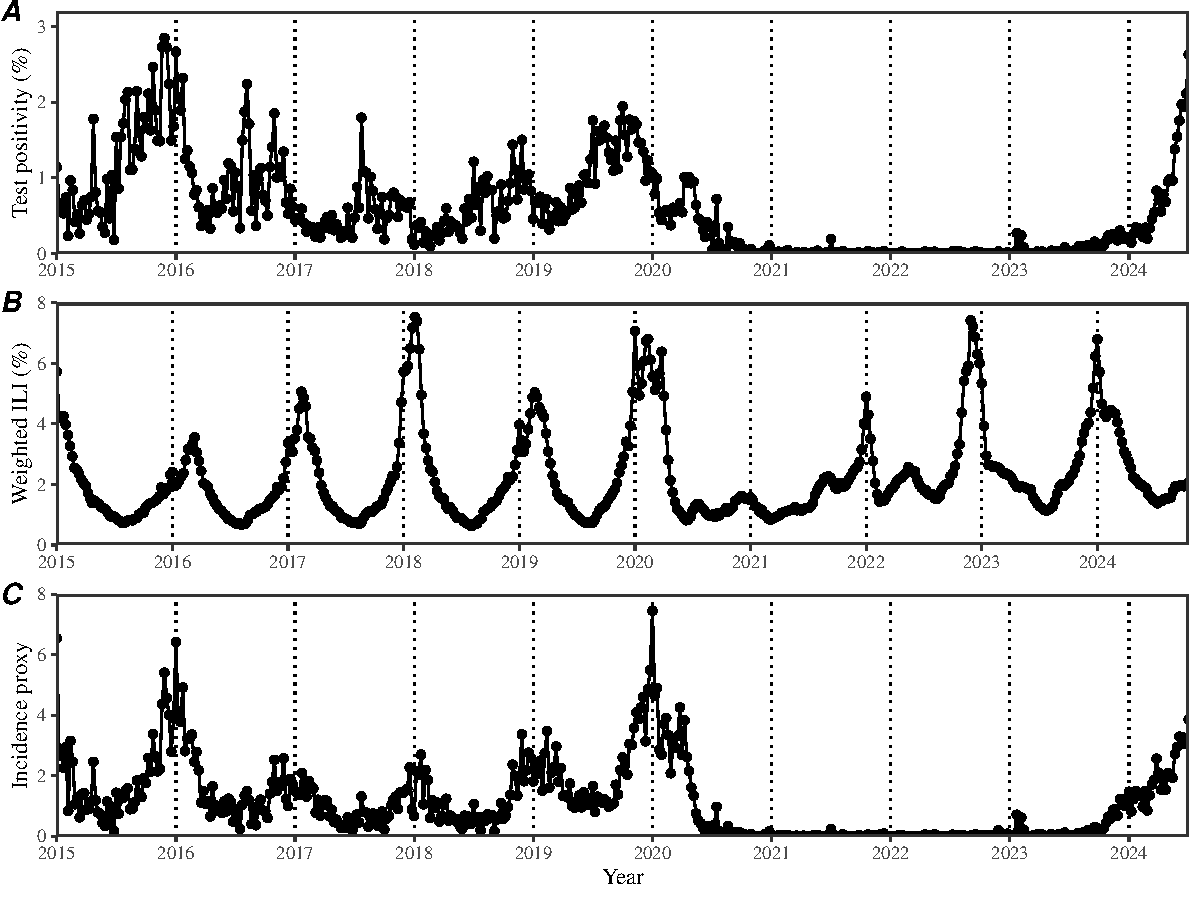
\includegraphics[width=\textwidth]{../figure_timeseries/figure_timeseries.pdf}
\caption{
\textbf{Comparisons of time series data.}
(A) Weekly percent positivity of Mp infections BIOFIRE® Respiratory Panel in the US.
(B) Weekly percent positivity of outpatient visits for ILI in the US.
(C) Estimated weekly incidence proxy.
}
\end{figure}

\pagebreak

\begin{figure}[!ht]
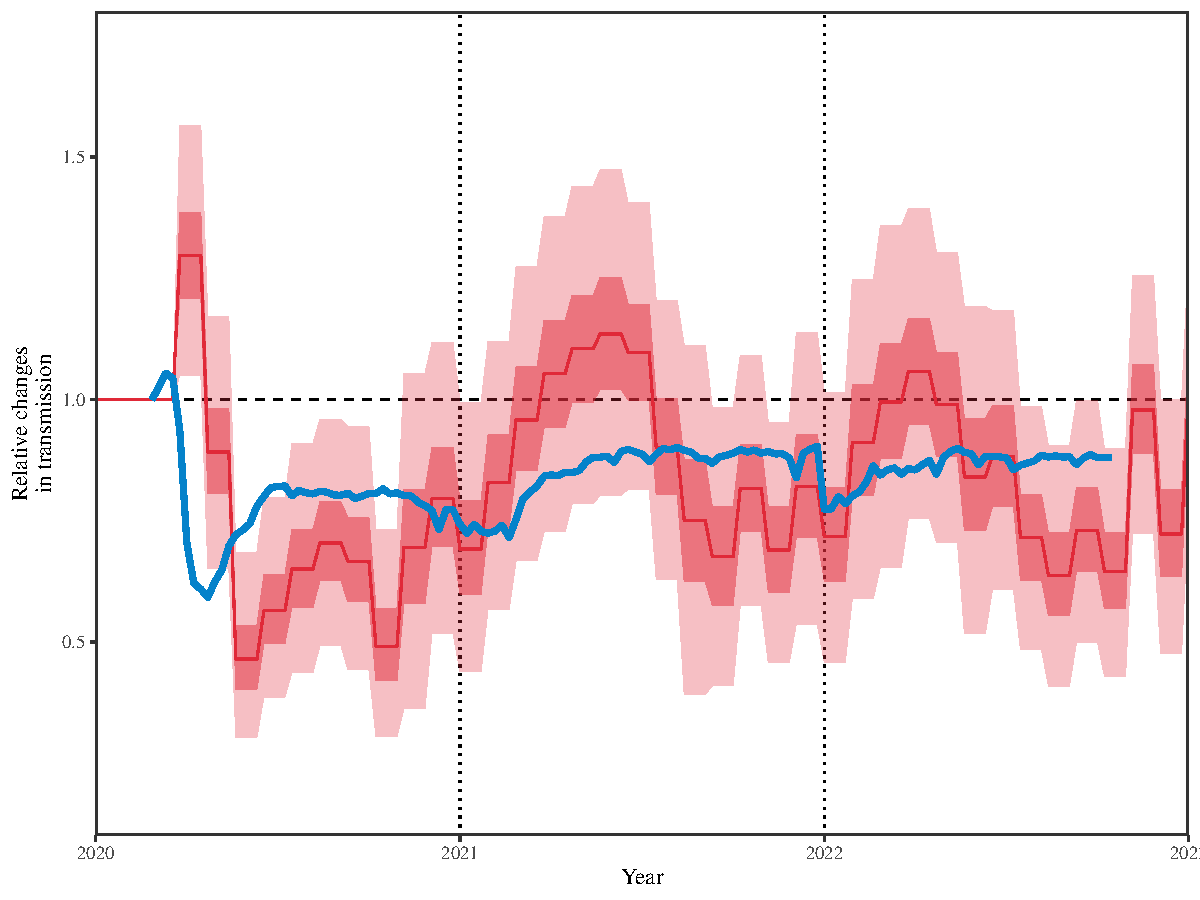
\includegraphics[width=\textwidth]{../figure_mobility/figure_mobility_new.pdf}
\caption{
\textbf{Comparisons of estimated changes in transmission (red) and mean Google mobility measures (blue).}
Mean mobility was calculated by taking the average mobility across four categories: retail \& recreation, grocery \& pharmacy, transit stations, and workplaces \citep{park2024predicting}.
}
\end{figure}


\pagebreak

\begin{figure}[!ht]
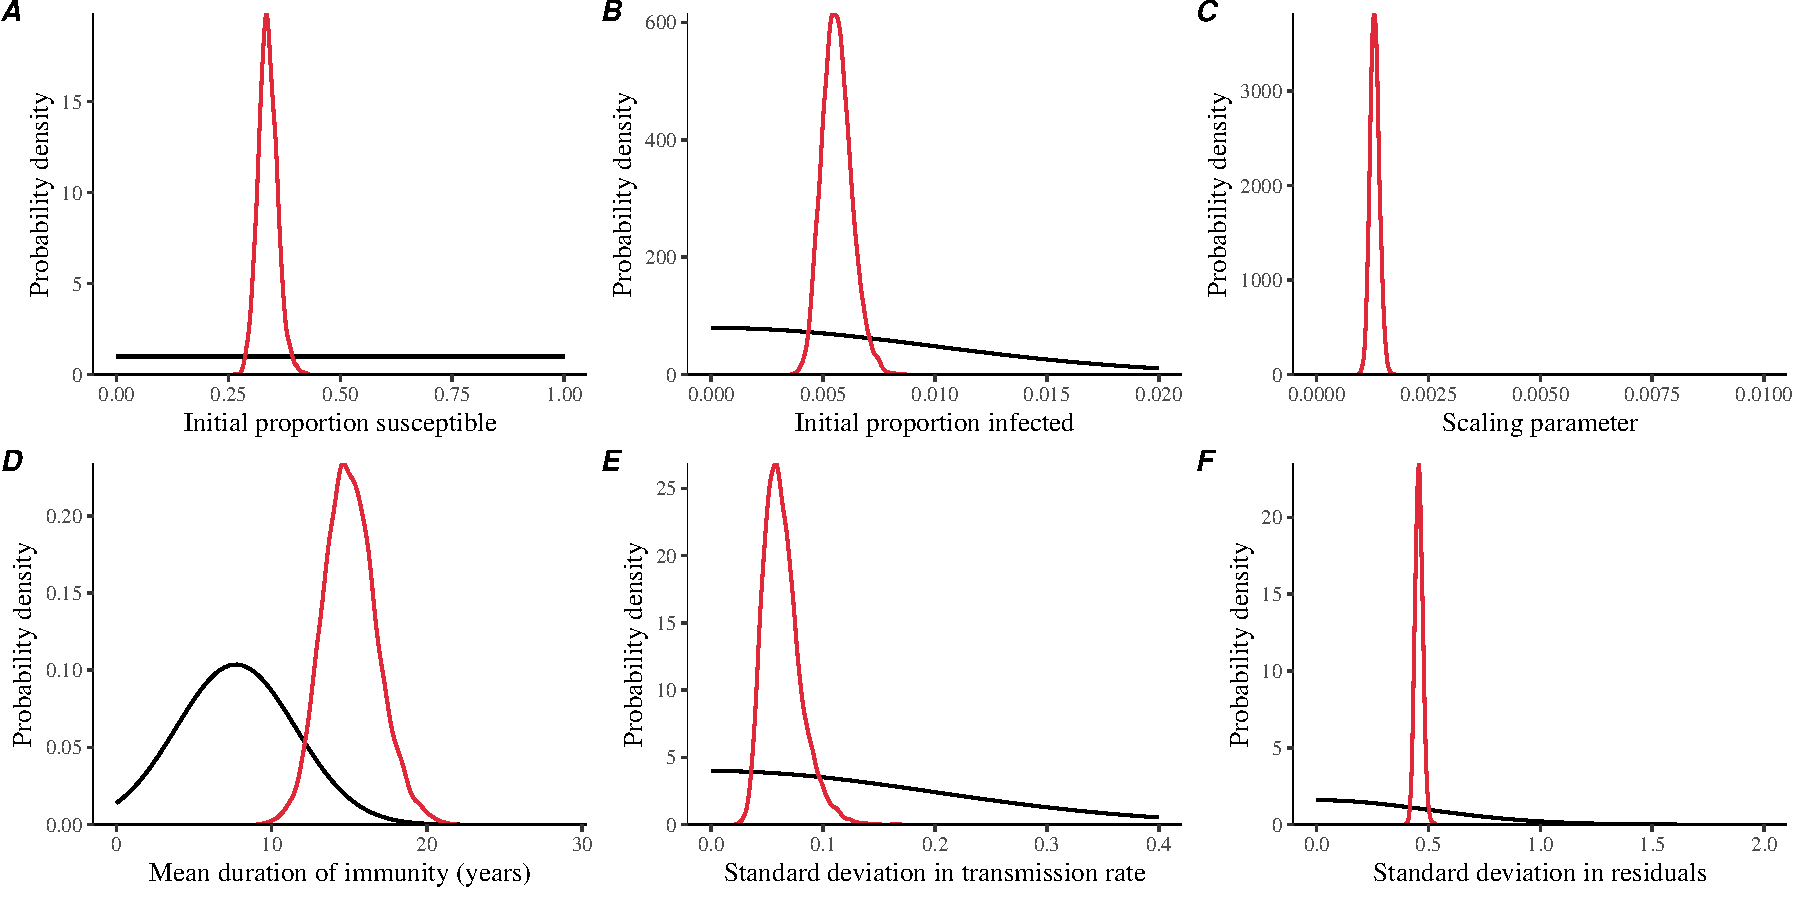
\includegraphics[width=\textwidth]{../figure1/figure1_posterior.pdf}
\caption{
\textbf{Comparisons between posterior and prior distributions.}
Black lines represent prior distributions.
Red lines represent posterior distributions.
Posterior distributions for the seasonal transmission rate and NPI effects are presented in Figure 1.
}
\end{figure}


\pagebreak

\begin{figure}[!ht]
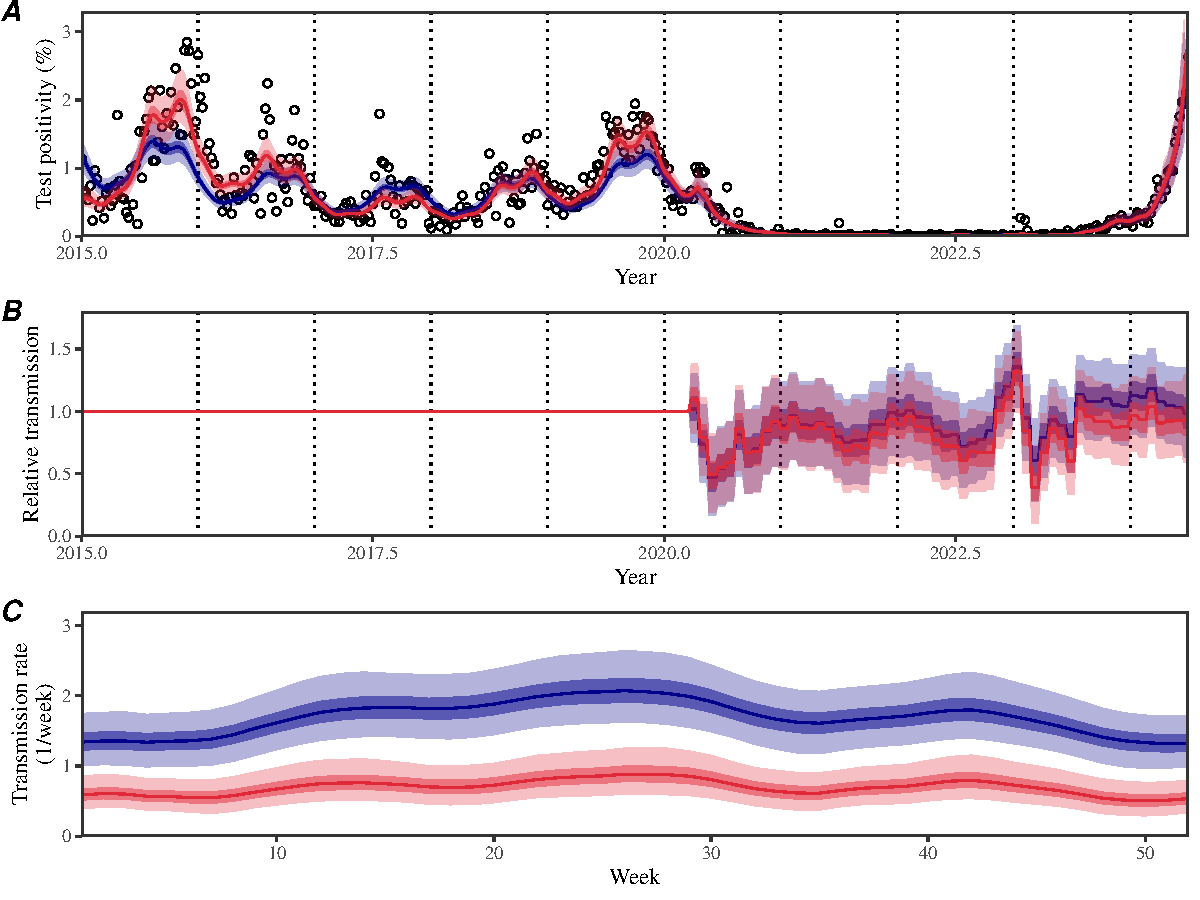
\includegraphics[width=\textwidth]{../figure_sirs/figure_sirs_fit.pdf}
\caption{
\textbf{Comparisons of SIRS (red) and SIR (blue) model fits to Mycoplasma pneumoniae positivity in the US, 2015--2024.}
(A) Comparisons of observed (points) and fitted (line) changes in weekly test positivity for Mp infections.
(B) Estimated non-periodic, time-varying transmission term, representing relative transmission $\delta$ following the introduction of NPIs.
These changes are relative to the seasonal transmission rate shown in panel C;
for example, 0.5 corresponds to a 50\% reduction in transmission.
(C) Estimated periodic transmission term  $\tsub{\beta}{seas}(t)$, representing seasonal transmission rate.
Lines and shaded regions represent the estimated posterior median and corresponding 95\% and 50\% credible intervals.
}
\end{figure}

\pagebreak

\bibliography{myco}

\end{document}
